\documentclass[10pt,letterpaper]{article}
\usepackage[utf8]{inputenc}
\usepackage{cite}
\usepackage{amsmath}
\usepackage{amsfonts}
\usepackage{amssymb}
\usepackage[left=2cm,right=2cm,top=2cm,bottom=2cm]{geometry}
\usepackage{graphicx}
\title{Anomaly Detection in Graphs}
\author{Coen Valk}
\begin{document}
\begin{huge}
\begin{center}
Anomaly Detection in Graphs\\
Coen Valk
\end{center}
\end{huge}
\section{Introduction}

Anomaly detection is an important topic in many fields including financial
fraud detection, event tracking, and network security to name a few.
Several methods for detecting anomalies have been created over the years, each
with its advantages and disadvantages. Here we will discuss the performance of
certain anomaly detection algorithms on a few different datasets to learn more
about the strengths and weaknesses of each algorithm.

\section{Background}

Anomalies can be found at several different scopes of a graph:

\begin{itemize}
	\item \textbf{Global:} Where each node is compared to every other node,
		without regard for graph structure.
	\item \textbf{Local:} Where each node is compared to its direct neighbors.
	\item \textbf{Community:} Where each node is compared to nodes in the same
		community.
\end{itemize}

Searching for anomalies at any of these three scopes may produce differing
results. For instance, if one were to have a graph of interactions between people
with node attributes on income, a global outlier detection method would consider
such high wealth individuals including Jeff Bezos and Bill Gates as anomalies.
However, within the context of the billionaires that Jeff Bezos and Bill Gates
typically interact with - by comparing nodes at the local or community scale -
their income might not be as anomalous as we had originally thought.

\subsection{GLODA}

the global outlier detection algorithm (GLODA) finds outliers without considering
graph structure. This is often done using the local outlier factor (LOF)
algorithm\cite{LOF}. LOF determines outliers by identifying how many
k-nearest neighbors are in common between nodes. if a node has few neighbors in
common with other nodes, it will be considered anomalous.

\begin{figure}[ht]
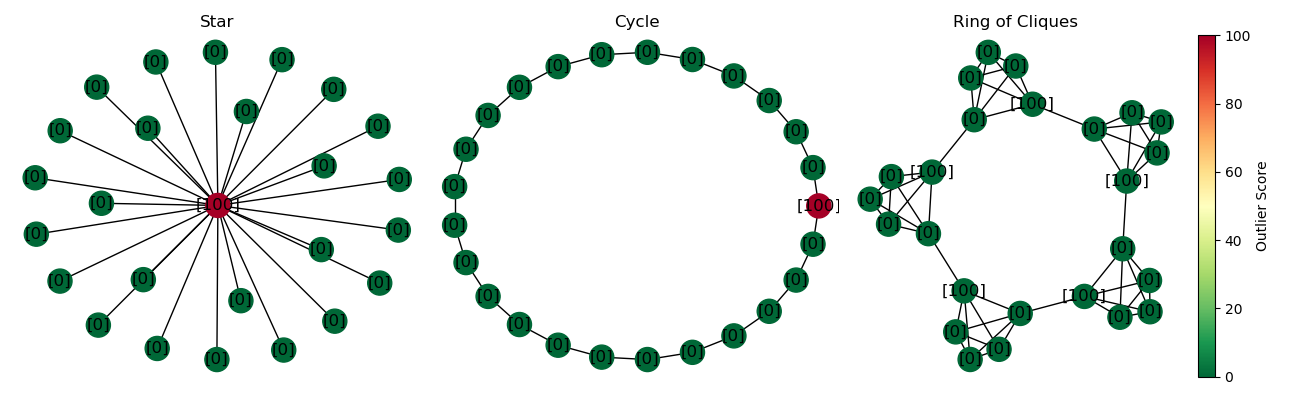
\includegraphics[width=\textwidth]{"../graphics/GLODAExample.png"}
\caption{GLODA outlier scores}
\end{figure}

Figure 1 shows how
GLODA determines outliers in three different graph topologies. Each node in the
figure is labeled with its attribute (in this case an array containing one value)
and colored with its corresponding outlier score. Observe that GLODA does not
find any anomalies in the ring of cliques example, as there are several nodes
with attribute 100, and without the graph context that might not seem peculiar.

\subsection{DNODA}

local outliers can be found using the direct neighbor outlier detection algorithm
(DNODA). It scores each node based on the average distance from its direct
neighbors given by the equation:

$$ \text{Score}(v) = \frac{ \sum_{u \in N_v} dist(u, v) }{|N_v|} $$
Where $N_v$ is the set of neighbors for node $v$.

\begin{figure}[ht]
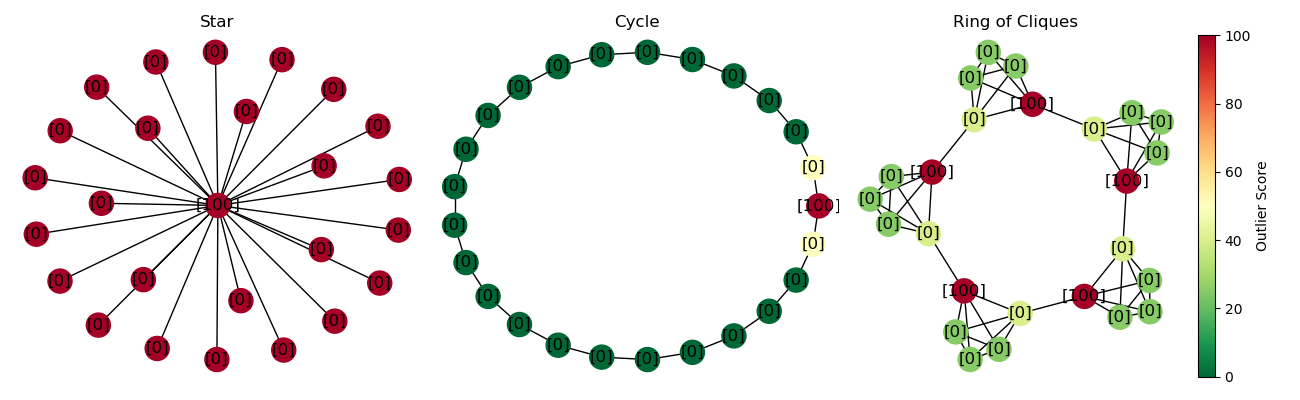
\includegraphics[width=\textwidth]{"../graphics/DNODAExample.png"}
\caption{DNODA outlier scores}
\end{figure}

Figure 2 shows DNODA's labeling on the three graphs. observe that the star graph is
labeled completely anomalous. Because each node is connected to the center, the mean
distance of neighbors is the same for each node - so each node is given a distance of
100. This result is not usable, and so all nodes would be considered not anomalous.
On the other hand, DNODA does well identifying anomalous nodes in the cycle and ring
of cliques structures.

\subsection{CNA}

The community neighbor algorithm (CNA) is very similar to DNODA except its scope
broadens to a community. CNA needs
to first perform a community detection algorithm to find clusters of nodes, then
for each node finds the average distance between itself and the rest of the nodes
in its community as shown in the equation:

$$ \text{Score}(v) = \frac{\sum_{u \in C_v} dist(u, v) }{|C_v|} $$
Where $C_v$ is the community that contains node $v$.

\begin{figure}[ht]
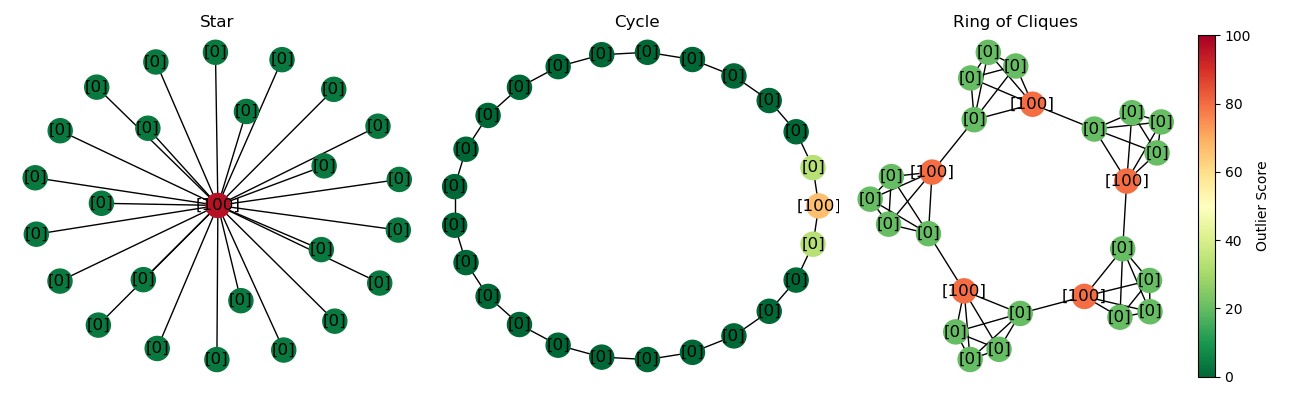
\includegraphics[width=\textwidth]{"../graphics/CNAExample.png"}
\caption{CNA outlier scores}
\end{figure}

Figure 3 shows CNA's labeling for each of the three graph structures. CNA identifies
anomalies in these three graph examples rather well.

\subsection{Oddball}

Another common method for anomaly detection as is used by the Oddball algorithm
is coming up with patterns in a dataset including relationships between nodes
and edges, edges and total edge weights. Deviations from this pattern could be
considered anomalous\cite{OddBall}. Oddball works on the theory that most
graphs exhibit power law relationships between certain graph attributes, even at
a local neighbor scale. Oddball performs this power law analysis on each node's
egonet - the subgraph containing all of a nodes direct neighbors and edges between
such neighbors. Oddball's outlier score function is

$$ \text{Score}(i) = \frac{\max(y_i, Cx_i^\theta)}{\min(y_i, Cx_i^\theta)} \cdot \log(|y_i - Cx_i^\theta| + 1) $$

Where $C, \theta$ are the best fit parameters that fit the power law relationship
between $x, y$.

As Oddball works on the assumption that the input graph exhibits power law relationships,
the three simple example graph topologies used to demonstrate performance
of GLODA, DNODA and CNA are not effective. Instead, we will construct a small graph that
does exhibit real-world observed power law relationships with respect to
egonet-density power law (EDPL) and edge-weight power law (EWPL) to showcase how
Oddball differs from GLODA, DNODA, and CNA\cite{RTM}.

\begin{figure}[ht]
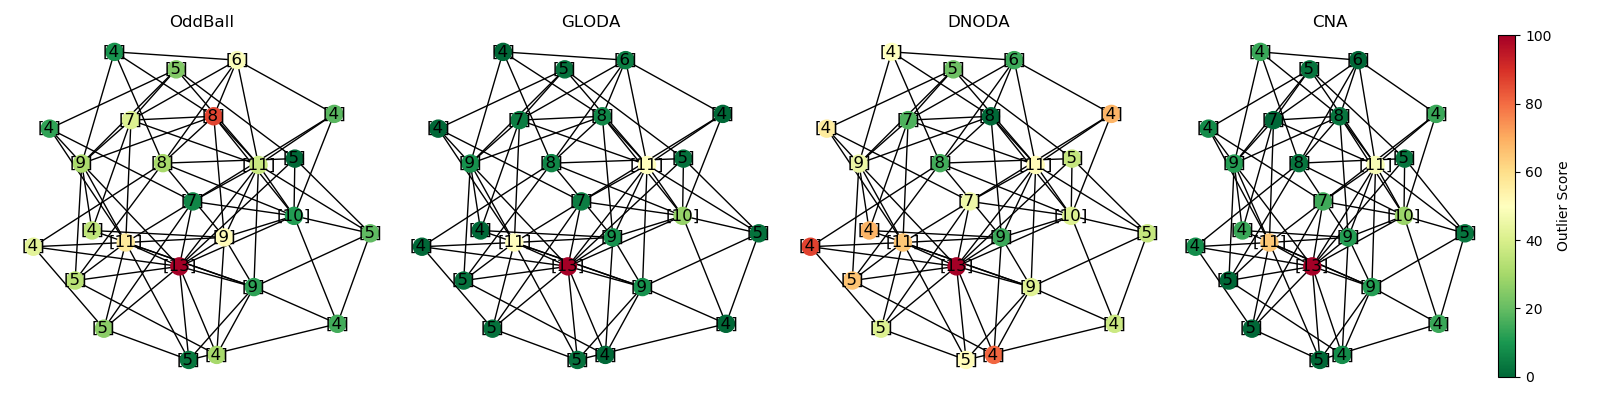
\includegraphics[width=\textwidth]{"../graphics/OddballExample.png"}
\caption{Oddball vs. GLODA, DNODA, and CNA}
\end{figure}

Observe in figure 4 how certain nodes are colored differently between
algorithms. Notably, the Oddball algorithm finds outliers that the other 3 algorithms do not pick up on. These are nodes that fall outside of the typical expectation of the power law in its egonet, but might not specifically be distant from other nodes.

\section{Methods}

Each algorithm will run on 3 datasets to identify nodes that all algorithms identify as 
anomalous and nodes that only one algorithm considers anomalous. Then we will combine
the results of all of these algorithms' rankings using the borda voting system
to come up with one list of anomalous nodes. Some information on the three datasets:

\begin{itemize}
\item \textbf{Enron:} Emails between executives at Enron.
\item \textbf{FEC donation data:} Federal Election Committee data of donations from individuals to political committees.
\item \textbf{Elliptical Bitcoin Transaction Data:} Financial transaction network
with labeled data on "illicit" nodes. The behavior of illicit nodes is more
nuanced than distance from the average.
\end{itemize}

Each of these algorithms are node-focused and GLODA, DNODA, and CNA depend on
distance between nodes to determine outlier scoe. Therefore each dataset has
features that need to be engineered slightly before each algorithm can run
properly on the data.

\subsection{Enron}

The only feature engineering for the Enron dataset for this example is the degree per
node. This will find anomalies that have significantly higher or lower degree
than the other nodes it is compared to. This will be necessary for GLODA, DNODA and
CNA to make inference on anomalies.

To match this outlier detection attempt, the Oddball algorithm will fit to
the edge density power law (EDPL) to find either near-cliques or near-stars.

\subsection{FEC Donation Data}

The FEC donation data has edge weights for donation amount. As mentioned
earlier however, these algorithms are node-focused. To account for this, each node will
have as attributes the mean and median donation from that node. This will find
nodes that have particularly large or particularly small donations compared
to similar nodes.

For the Oddball algorithm, we will fit to the edge-weight power law (EWPL)
to find similar anomalies in the graph.

As an added note, if it is necessary to do anomaly detection on edges like in
credit card fraud detection, one may perform the same anomaly detection algorithms
on the induced line graph of the data. Unfortunately with large hubs such as in the 
donation network, a line graph will have large cliques which are prohibitively
expensive to work with. For this example we will stick with data from the original
graph structure.

\subsection{Bitcoin Transaction Data}

The Bitcoin transaction dataset has more than 100 numerical attributes per node.
To save on compute time the dataset is reduced using principal component analysis
(PCA) while keeping 80\% of the variance. This reduces the dimensionality all the
way to 13 numeric attributes per node.

\section{Results}

\subsection{Enron}

\begin{verbatim}
Enron Worst Offenders:
  GLODA: [4938 3994 6374 8876 2598  280    1 6211 1356 3982 4406 1470 4281 1394
 4283 2375  159  992 3052  821] 0:00:02.054511
  DNODA: [27137 27167 27148 27150 27164 27163 27162 27161 27160 27159 27149 27158
 27156 27155 27154 27153 27152 27151 27157 27646] 0:00:01.233046
  CNA: [ 107   97   95  188  244   89  182   93 1273   96   92   79  148  245
   85  197   80  191  144  271] 0:00:21.412095
  OddBall: [34257 21043 32192 33284 30623 36248 34797 36640 30609 35234 33276   224
 22412 36324   271 36311   153 36297 20260 32713] 0:00:14.729157
    Borda: [244  96 148 153 119 197  80 191 144 271]
Done.
\end{verbatim}

Above are the top 20 outliers for each algorithm when run on the Enron dataset
along with the result after
ranking with borda. Notice that there are a couple similarities between the outputs
of each algorithm. It seems that in this example, the community neighbor algorithm
performed well by identifying anomalous nodes that were generally agreed upon by
all of the algorithms to be outliers.

\subsection{FEC Donation Data}

\begin{verbatim}
FEC Donation Data Worst Offenders:
  GLODA: [   55 34519 60281 60737 20017 50180  1675  2558 14665 56009  2060 34646
 29594 36236 43165 41717 25511 54672 28561 43911] 0:00:03.711894
  DNODA: [30013 29406 60907  6780 28342 31234 42065 15983 10335 57382 23679 67106
 67695 29179 48156 67911 14308  9859 46801  4893] 0:00:00.981846
  CNA: [28342 10335  7186 54303 29179 48156 67911 57382 30013  6780 31234 15983
 42065 23679 67695 67106  4893 46801 14308  9859] 0:05:31.636945
  OddBall: [50548  9825 21396 21340 67695 17148 29301 44857  1480 67911 29179 48156
 28342  3574 47968 47862 29406 60907 46801  4893] 0:11:41.377449
  Borda: [25664 56528 45919  8450 49473 49891   233 25511  9822 22647]
Done.
\end{verbatim}

In this example, DNODA and Oddball most notably have some identified nodes in common,
albeit in a slightly different order. Beyond this, there are no node ids that
stand out as being in every algorithm's list of highest outlier score.

\subsection{Bitcoin Transaction Data}

\begin{verbatim}
Bitcoin Data Worst Offenders:
  GLODA: [132852  17622   4265 133605  12532  11652  11025 129090 134619   7215
   6391 128164 127304   4486   3378   5913   7521   1376   1661 136165] 0:00:36.455671
  DNODA: [191731 192356 190412 192608 193037 193137 192737 192039 192919 192728
 192504 192282 192021 190783 144268 192979 193021 140237 140236 141690] 0:00:03.762974
  CNA: [144268 144269 115222 126218 116671 111866 111967 127239  63415 203550
 193603 126265 126344 140236 141690 127504 126639 189851 197761 140237] 0:16:15.680851
  OddBall: [192039 190412 192356 191596 192015 192919 192282 190783 191731 192737
 193021 192728 192608 193137 193037 192979 192504 130048 140236 141690] 0:00:29.681412
  Borda: [126344 197761 115008 126639 127504 126517 126265 140237 140236 141690]
Done.
\end{verbatim}

This dataset showed the most consistent results, with certain nodes being in almost
all of the algorithm's top 20 outliers. This results in a borda count very similar
to both Oddball as well as DNODA.

\section{Conclusion}

Ultimately, each algorithm does not necessarily perform "better" or "worse" than any of 
the others, but simply looks for different kinds of anomalies, and at times all
of these algorithms produce similar results. The use of any of these
algorithms is determined mostly by the user's needs and what kind of anomalous
behavior they are looking for.

\bibliography{bib}{}
\bibliographystyle{plain}
\end{document}